\documentclass{vivid_layout_pdf}

%% Required to build cover page
\title{Everything You Need To Know About}{Queueing Theory}
\date{\today{} \textbullet{} Revision 2}
\cover{queueing-theory/cover}

%% Required to build "Meet the Author"
\author{Baron Schwartz}{img/baron}

%% Required image for "About VividCortex"
\aboutvc{img/presenter}

%% Required resource info
\resourceleft%
	{The Strategic IT Manager's Guide To Building A Scalable DBA Team}
	{}
	{img/scalable-dba-team}
	{https://www.vividcortex.com/resources/building-scalable-dba-team/}
\resourceright%
	{Case Study: SendGrid}
	{VividCortex has been instrumental in finding issues. It's the go-to solution for seeing what's happening in production systems.}
	{img/sendgrid-thumbnail}
	{https://www.vividcortex.com/resources/case-studies/sendgrid/}

\begin{document}
\maketitle		% Build the cover page
\begin{bio}		% Biographical info for "Meet the Author"
Baron is well-known for his contributions to the MySQL, PostgreSQL, and Oracle communities. Baron has helped build and optimize database systems for some of the largest Internet properties. He has written several books, including O'Reilly's best-selling High Performance MySQL. Prior to founding VividCortex, Baron managed consulting, support, training, and software engineering at Percona. He has a CS degree from the University of Virginia.
\end{bio}
\tableofcontents	% Build the table of contents

\section{Queueing Theory is for Everyone}

Whether you're an entrepreneur, engineer, or manager, learning about queueing theory is one of the best ways to boost your performance. Queueing theory is fundamental to getting good return on your efforts. That's because the results your systems and teams produce are heavily influenced by how much waiting takes place, and waiting is waste. Minimizing this waste is extremely important. It's one of the biggest levers you will ever find for improving the cost and performance of your teams and systems.

Unfortunately, queueing theory books are often terribly complicated and boring. But it doesn't have to be that way! The concepts are easy to understand, and developing intuition about what happens in queues is the real low-hanging fruit. Plus, queueing theory is super-cool, and it's a pity if you don't learn about it.

There are plenty of 350-page books about queueing theory, and lots of high-level introductions too. But these all either dive deep into pages full of equations and Greek symbols, or gloss over (or just outright lie about) the big, important truths of queueing. We need a middle ground.

My hope is that this book can help you achieve the following:

\begin{itemize}
\item Develop awareness of how queueing appears in everyday life. Queueing rules everything around you, but many people probably aren't aware of it.
\item Build intuition of important concepts and truths that can guide you in decision making.
\item Help you see where your intuition is a trusty guide and where queueing will surprise you.
\item Help you understand the landscape of queueing theory from a general framework, so you can quickly navigate more detailed treatises and find the right answers fast.
\end{itemize}

Armed with the knowledge in this book, you will be able to quickly understand common scenarios such as:

\begin{itemize}
\item If web traffic increases 30\%, will the server get overloaded?
\item Should I buy faster disks, or should I just buy a few more of what I already have?
\item What if I specialize tasks in my team and create a handoff between roles?
\end{itemize}

Knowing how to think about these kinds of questions will help you anticipate bottlenecks. As a result, you'll build your systems and teams to be more efficient, more scalable, higher performance, lower cost, and ultimately provide better service both for yourself and for your customers. And when you need to calculate exactly how much things will bottleneck and how much performance will suffer, you'll know how to do that too.

As for scope, the aim of this book is to help you get answers for common scenarios and point you to the right resources for other cases. I'll go into details where they help illuminate important concepts.

I'll also try to make it fun in a nerdy way. In the end, I hope the Aaron Neville and Linda Ronstadt song will take on new meaning for you:

\begin{quote}
Don't know much\newline
But I know I love queues\newline
And that may be\newline
All I need to know
\end{quote}

\section{What is Queueing Theory?}

Queueing theory is a broad field of study that focuses on the many nuances of how waiting lines behave. It's a fascinating topic if you're of a theoretical bent. But it's highly relevant even if you're the impatient ``just answer my question!'' type, too.

Queueing theory boils down to answering simple questions like the following:

\begin{itemize}
\item How likely is it that things will queue up and wait in line?
\item How long will the line be?
\item How long will the wait be?
\item How busy will the server/person/system servicing the line be?
\item How much capacity is needed to meet an expected level of demand?
\end{itemize}

These questions can easily be rephrased and used to answer other questions, such as ``how likely am I to lose business due to too-long waits or not enough capacity?'' and ``how much more demand can we satisfy without creating an unacceptably long wait?''

And although I wrote the questions in simple terms, you can also answer sophisticated questions about the characteristics of the answers. For example, ``how long will the wait be?'' can be answered not only on average, but you can calculate things such as the variability of wait times, the distribution of wait times and how likely it is that someone will get extremely poor service, and so on.

\section{Why Queueing Theory is Tricky}

Bad news: queueing theory is part of probability theory, and probability is hard and weird. Nothing leads you astray faster than trusting your intuition about probability. If your intuition worked, casinos would all go out of business, and your insurance rates would seem reasonable.

In particular, human intuition is {\itshape linear}. Double the traffic, we think, and other things will double too. {\itshape Wrong!} Queueing systems are {\itshape nonlinear}. What's worse is that they're unpredictably nonlinear. Things seem to change gradually, until you reach some tipping point and {\itshape boom}, everything gets really bad, really fast. These transitions can be so sudden that they are very surprising. Our intuition isn't geared to expect these disproportionate, sudden changes.

The classic example you might recognize is the so-called hockey-stick curve. We need a picture to break up all this text, so I'll introduce that now. This is the most famous queueing theory picture of all time:

\begin{center}
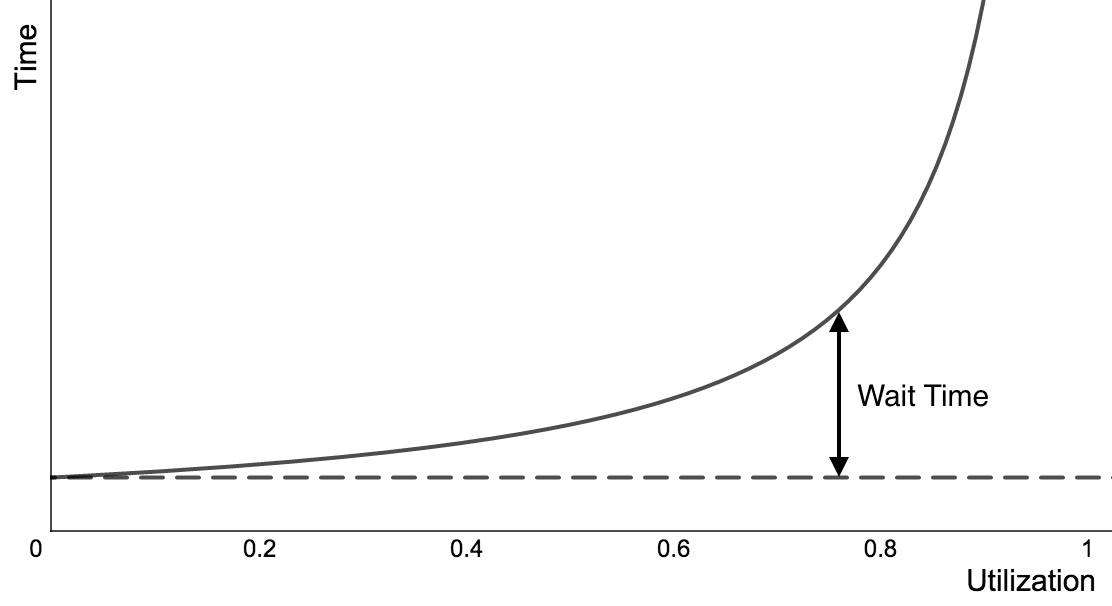
\includegraphics[width=.75\linewidth]{queueing-theory/hockey-stick-1}
\end{center}

This curve shows how a system's total response time increases as utilization increases. As utilization approaches 100\%, response time goes to infinity. The exact shape of this curve depends on the characteristics of the system and the work it's doing, but the general principle applies to pretty much all systems.

You'll get familiar with nonlinearity over the course of this book. You might never be able to accurately estimate {\itshape how much} things will be nonlinear. But you'll get pretty good at recognizing situations where someone needs to check whether bad stuff is going to happen. Then you'll do a little bit of math or look things up in a table and find the answers you need.

\section{Queueing Systems in Real Life}	% A section heading

Most introductions to queueing theory talk about abstract things and use jargon a lot. They'll usually discuss some real-life scenarios to help you understand the abstract things, but for some reason they always seem to pick bizarre situations I personally have never encountered\footnote{Often with British terminology, something about hiring lorries and abseiling}. Then they jump into discussions of Markovian something or other, and talk about births and deaths. At this point my eyes have usually glazed over.

But life is full of queueing systems!
\begin{itemize}		% Create a bulleted list
\item Your Kanban board
\item Getting a latte at the coffee shop
\item The line for the restroom after drinking the latte
\item Your computer's CPUs and disks
\item At the traffic light
\item When the captain says you're third in line for takeoff
\item Your load balancer
\item Pre-ordering the new iPhone
\item Trying to pick the best line at the grocery checkout counter
\item Merging onto the freeway
\item Connection pooling
\end{itemize}

Importantly, queueing systems are present in much more subtle scenarios too. Any process for handling units of work has queueing systems built into it. When you ask your graphic designer to produce a beautiful new ebook, for example (ahem), queueing is at work.

One of the big wins is being able to recognize these systems, particularly in {\itshape teams}. Teams have communication structures, and communication---whether it's email or chat at the water cooler---is queueing. Send an email to your colleague; when it's in their inbox it's queued. If a developer doesn't know how to optimize a query and asks a DBA for help, and the DBA is busy, the developer's request is queued. Design your organization with the recognition that {\itshape teams are systems too}, and you'll have a chance to get much better results.

\section{Why Does Queueing Happen?}

Why do things wait in queues anyway?

It might seem like a dumb question with an obvious answer. ``Because there's more work to do than capacity to do it, silly!'' But that is not the right answer. Queueing happens even when there's more than enough capacity to do the work. This is part of what's really surprising and counterintuitive about queueing theory. This is so important that it needs to be emphasized:

\begin{quote}
Queueing happens even when there's more than enough capacity to do the work.
\end{quote}

Let's take a simple example. Suppose a grocery store has a single checkout line and a single cashier. Suppose an average of one shopper per minute arrives at the line to pay for their groceries. Scanning, bagging and paying takes 45 seconds on average. Will there be queueing and waiting?

Intuition says no, there won't. There will be, on average, 15 seconds of idle time for the cashier every minute. The cashier is only busy 75\% of the time! Of course no one has to wait in line, right?

But that's not what really happens. In reality, there will be lots of shoppers waiting in line and they'll have to wait a long time!

Why on earth would this happen? It seems to make no sense at all.

Fundamentally, queueing happens because of three reasons:
\begin{enumerate}	% Create a numbered list
\item {\bfseries Irregular arrivals.} Shoppers don't arrive at the checkout line on a regular schedule. They're sometimes spaced far apart and sometimes
close together, so they overlap. An overlap automatically causes
queueing and waiting.
\item {\bfseries Irregular job sizes.} Shoppers don't all complete in 45 seconds.
Some of them will take much longer. And when this happens, there's
overlap again because new shoppers will arrive and be ready to
check out while the existing ones are still in progress.
\item {\bfseries Waste.} Lost time can never be regained. Shoppers who arrive at the line just after someone else overlap because the first shopper didn't have time to finish. But if you look at it another way, perhaps it's not the second shopper's fault. Perhaps the first shopper should have arrived earlier, but wasted time doing something else while the cashier was idle! They missed their chance and made the second shopper have to wait. When the cashier is idle, time is wasting, and can never be gotten back because the cashier can't be more than 100\% utilized. Everything gets delayed permanently, and that shows up as queueing for later arrivals.
\end{enumerate}
In general, irregular arrival times and irregular job sizes are guaranteed to cause queueing.  The only time there's no queueing is when the job sizes are uniform, the arrivals are timed evenly, and there's not too much work for the cashier to keep up. Even when the cashier is not busy at all, irregular or bursty arrivals will cause some queueing.

Queueing gets worse when the following are true:

\begin{itemize}
\item {\bfseries High Utilization.} The busier the cashier is, the longer it takes to recover from wasted time.
\item {\bfseries High Variability.} The more variability\footnote{If you've read Eli Goldratt's {\itshape The Goal}, you should recognize the phrase ``statistical variations.'' This book is all about queueing theory even though it doesn't mention it explicitly. The same is true for {\itshape The Phoenix Project} by Gene Kim et al.} in arrivals or job sizes, the more waste and the more overlap (queueing) occurs.
\item {\bfseries Few Servers.} Fewer cashiers means less capacity to absorb spikes of arrivals, leading to more wasted time and higher utilization.
\end{itemize}

\section{The Queueing Theory Framework}

All discussions of queueing theory analyze systems and processes in terms of three key concepts:

\begin{itemize}
\item {\bfseries Customers} are the units of work that the system serves. A customer can be a real person, or it can be whatever the system is supposed to process and complete: a web request, a database query, a part to be milled by a machine.
\item {\bfseries Servers} are the things that do the work. This might be the cashier at the grocery store, the web server or database server, or the milling machine.
\item {\bfseries Queues} are where the units of work wait if the server is busy and can't do the work as it arrives.
\end{itemize}

These are abstract concepts that can be extended to every situation. There are also variations on the names. For example, servers are sometimes called ``stations,'' and sometimes I'll call a customer a ``job'' or ``task'' in this book.

Queueing theory views every system as interconnected sets of servers and queues, through which customers flow. Graphically, queues are represented as a set of stacked boxes, and servers/stations are shown as circles.  The simplest possible system is a single queue leading to a single server:

\begin{center}
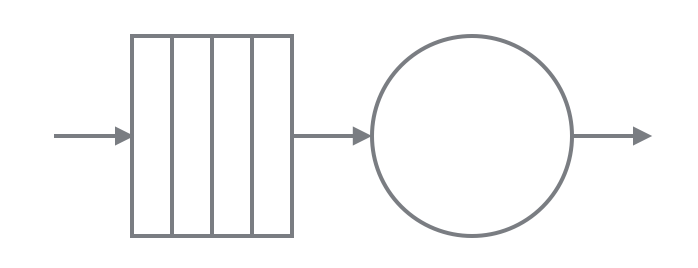
\includegraphics[width=.375\linewidth]{queueing-theory/queue-and-server}
\end{center}

However, it's possible to have a variety of configurations, such as 1-to-many, many-to-many, many one-to-one, and chained systems:

\begin{center}
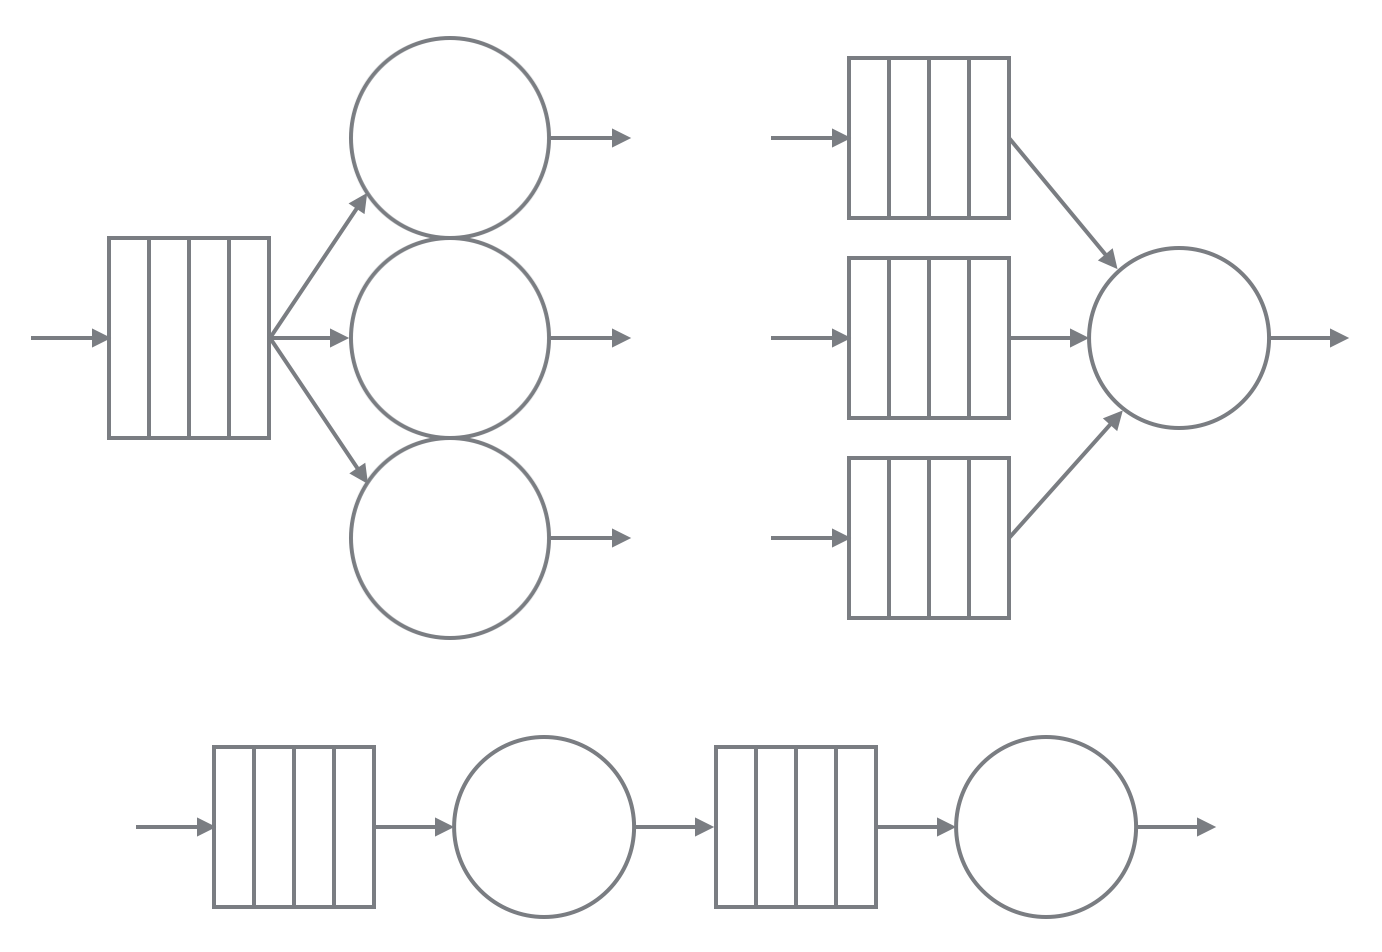
\includegraphics[width=.75\linewidth]{queueing-theory/queue-configurations}
\end{center}

Once you're aware of this framework, you can decompose any system into networks of queues and servers and analyze them individually or separately.

Now that you know that, what can you measure, analyze and predict about a queueing system?  There are a variety of important metrics and parameters:
\begin{table}{X[-1,l,m]|X[-1,l,m]|X[-1,c,m]|X[-3,l,m]}
{\bfseries Metrics} & {\bfseries Units} & {\bfseries Symbol} & {\bfseries Description} \\
Arrival Rate & Customers per time & $\lambda$ or $A$ & How often new customers arrive at the front of the queue. In a stable system that will reach equilibrium, this is the same as the completion rate, also called the throughput (sometimes denoted $X$). \\
Queue Length & Customers & $L_q$ & The average number of customers waiting in the queue. \\
Wait Time & Time & $W_q$ or $W$ & How long customers have to wait in the queue, on average. \\
Service Time & Time & $S$ & How long it takes to service customers after they leave the queue, on average. \\
Service Rate & Services per time & $\mu$ & This is the inverse of service time. \\
Residence Time & Time & $R$ & How long customers are in the system
overall, on average. In computer systems we usually call this latency or response time. It's the sum of wait time and service time. \\
Utilization & Fraction & $\rho$ or $U$ & How much of the time the system is busy serving requests. If the system has multiple servers, it's an average over all of them. This ranges from 0 to 1, inclusive. \\
Concurrency & Customers & $L$ & The number of customers waiting or in service, on average \\
Number of Servers & Servers & $M$ & The number of servers the system has (e.g. cashiers, CPUs). \\
\end{table}

You will find many different names used to describe some of these. There is no universal standard for naming or symbols, and I have only listed some of the most common ones. You will find others in use, such as sojourn times and delays, sometimes ambiguously. You'll also find different letters and symbols; for example, sometimes $s$ is the symbol for the number of servers.

The results you'll get from queueing theory are mostly about long-term averages in stable systems that reach equilibrium. A stable system is one that is able to keep up with all the incoming work, so all customers eventually get serviced, and queues don't grow to infinity.

Many of these parameters are related through a set of simple laws that are easy to understand. (Parts of queueing theory actually do make sense!) The most important of these is Little's Law, which explains the relationship between a few of the key metrics. It is important to note that Little's Law applies only to stable systems. In general, and with no further assumptions needed about any of the metrics, Little's Law states that
\[
   L = \lambda R
\]

In words, concurrency (the number of customers in the system) is arrival rate\footnote{Or throughput, or departures; in a stable system these are equal in the long term.} times residence time. This relationship can be solved for different variables and used to analyze all or part of a queueing system. For example, you can analyze just the queue:
\[
  L_q = \lambda  W_q
\]

You will find Little's Law in different guises absolutely everywhere. Another useful relationship is the Utilization Law, which states that utilization is throughput times service time:
\[
 \rho = \lambda  S
\]

Or, if you have $M$ number of servers,
\[
 \rho = \frac{ \lambda S }{M}
\]

Another way to compute utilization:
\[
 \rho = \frac{\lambda}{ \mu}
\]

Although they're simple, these formulas are pretty easy to apply incorrectly, so always be sure you double check everything. There are also some subtleties that trip me up repeatedly. For example, the queue length is by definition the number of customers in the queue only and not in service, but the wait time in the queue will include some time for the current customer in service to finish.

The utilization formula \(\rho = \lambda / \mu\) is notable because it shows directly what is intuitively clear: if customers are arriving faster than they can be served, then utilization will be more than 100\%, the queue will grow to infinity, and the system isn't stable.

Another extremely important equation is the relationship between residence time, wait time, and  service time:
\[
 R = W_q + S
\]

Residence time in a queueing system is usually what you'd think of as response time or latency. As this equation shows, it's the sum of two components.  Here's our earlier diagram showing the components again:

\begin{center}
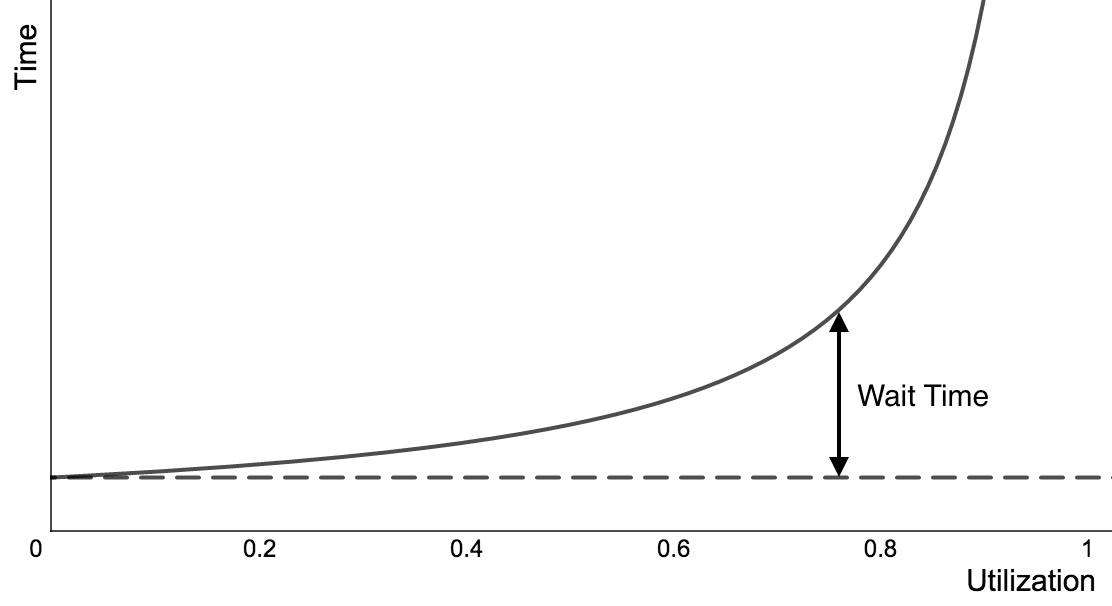
\includegraphics[width=.75\linewidth]{queueing-theory/hockey-stick-1}
\end{center}

The dashed line in this chart is the service time, which is a floor on how quickly a request will complete, on average. Even with zero queueing, the service time takes some minimal amount of time. The wait time in the queue is responsible for the hockey stick curve. Later I'll show you how to calculate that.

\section{Describing Queueing Systems}

As you have seen, there are different kinds of queueing systems, depending on how many queues and servers there are, and how they're connected together. Various configurations of queueing systems are typically described with Kendall's Notation, which gives a convenient shorthand for labeling classes of systems.

These are important because different kinds of systems have very different queueing behavior, which sometimes results in drastically different wait times and queue lengths. If you're going to analyze them, you'll need to be sure you know what kind of system you're working with, so you can pick the right analytical tools.

Kendall's Notation makes that easy. It is a set of slash-delimited letters and numbers that indicates the following:

\begin{itemize}
\item How arrival rates behave
\item How service times behave
\item The number of servers
\item Special parameters that are only needed in unusual cases and are usually left off. Just so you know what they are, they relate to whether the system has finite capacity and might reject arrivals, how big the population of customers is, and whether the queue does anything special to select which customer gets service next.
\end{itemize}

You'll commonly see a few kinds of queueing systems in Kendall's Notation:

\begin{itemize}
\item M/M/1
\item M/M/m (sometimes called M/M/c)
\item M/G/1
\item M/G/m
\end{itemize}

These letters mean the following.

\begin{itemize}
\item In the first position, the arrival rate is almost always specified as M, which stands for Markovian or Memoryless. This means that the customers arrive randomly and independently of each other, with average rate \( \lambda \). These arrival events are said to be generated by a Poisson process, and the time between arrivals is exponentially distributed, with mean \( 1/\lambda \).
\item The second position describes how the service times are distributed---that is, how long it takes to service each customer, with mean \( \mu \). This is often M as well, which means they are exponentially distributed, but sometimes it is G, which means the distribution is ``general'' and no specific distribution is assumed. Sometimes you'll see authors assume a Gaussian (normal) distribution, but it doesn't have to be Gaussian.
\item In the third place, you will find the number of servers. It'll either be an exact number, such as M/M/1 where there's explicitly 1 server, or you'll see an $m$ or $c$ as a variable placeholder, meaning a generalized system is being discussed and you'll plug the number of servers into the analysis.
\end{itemize}

The exponential distribution is very common in queueing analysis. Not only does it seem to describe real-world systems quite often, but it has nice mathematical properties that simplify analysis, and it's the safest bet when the real distribution is unknown. If you're not familiar with it, here's a chart of the exponential distribution's probability density function (PDF):\footnote{The PDF is what you get when you plot a histogram of a distribution.}

\begin{center}
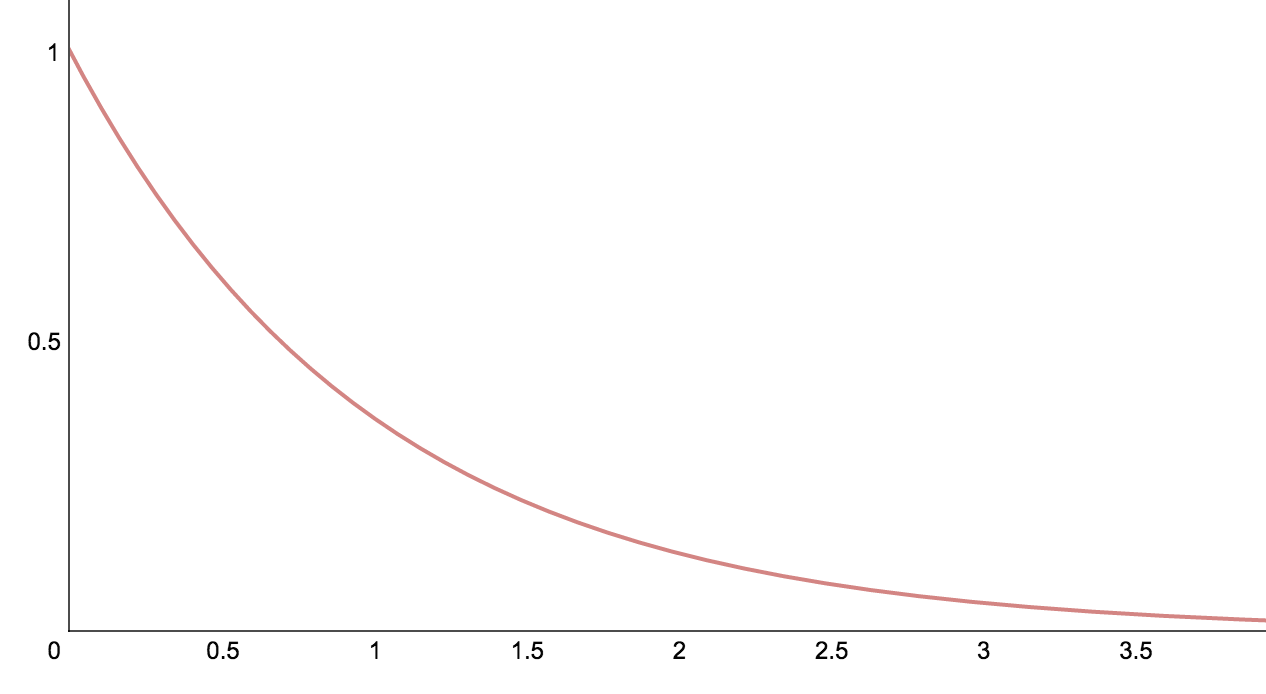
\includegraphics[width=.75\linewidth]{queueing-theory/exp}
\end{center}

Most of the time you'll work with M/M/m queuing systems. Lots of real-life situations are known to result in independent and randomly spaced arrivals, and it's usually a pretty safe default assumption unless you know otherwise. And if you think about it, lots of real-life service times are sort of exponentially distributed too, with most jobs completing pretty quickly but occasional outliers taking a long time.

Let's think about a few kinds of queueing systems and see what they are.

\begin{itemize}
\item The line at my local coffee shop is M/M/2. There's a single line, and people arrive randomly and independently (well, mostly... sometimes a few people arrive together), so that's an M. Their orders usually are pretty quick, but as you know, occasionally someone has trouble making up their mind and it takes a really long time, so M seems appropriate for the second letter. And there are two cashiers.
\item The security area at my local airport is best described as multiple M/M/1 queues. This applies to the ID check process as well as the bag check. In both cases I get in a line and I can't jump into an adjacent one, and there's a single person or single X-ray belt servicing me.
\end{itemize}

The M/M/m queueing system, and the exponential distribution, is sort of the moral equivalent of the Gaussian (normal) distribution in statistics. It shows up everywhere, it's nice to work with it, and it's well analyzed.

\section{Calculating Queue Lengths and Wait Times}

The usual use for queueing analysis is to answer questions about queue lengths and wait times. There are lots of other reasons to apply queueing theory, too, such as minimizing total cost of service and the like. But many of these applications center around queue lengths and wait times.

As I showed earlier, both queue lengths and wait times go to infinity as a server gets close to 100\% utilization. But what, exactly, is the shape of that hockey stick curve? How do you calculate it?

Finding exact answers can be tricky, because you have to figure out what kind of system you're dealing with. In the simplest M/M/1 case, your total time checking out is:
\[
  R = \frac{S}{1 - \rho}
\]

Therefore, your residence time is proportional to \( 1/(1-\rho) \), which is known as the {\itshape stretch factor}, a normalized measure of how ``stretched'' your residence time is relative to your service time. It is easy to see that this is an exponential curve; in fact it's the hockey stick curve. You can experiment interactively with it on \href{https://www.desmos.com/calculator/vhvwh6vjo7}{Desmos}.

Notice that the residence time doubles with every halving of \( 1-\rho \). If \( S = 0.25 \), for example, then

\begin{itemize}
\item At 50\% utilization, \( R \) is 0.5
\item At 75\% it is 1.0
\item At 87.5\% it is 2.0
\item And so on.
\end{itemize}

This leads to a useful rule of thumb to remember for a single-server queueing system: {\itshape residence time is inversely proportional to the server's idle capacity}. Halve the idle capacity, double the response time.

Note that if you want to determine any other desired metric about the queueing system, the laws given above make it possible. For example, if you want to calculate the queue length at a given utilization, you can find the time in the queue by just rearranging Little's Law, the Utilization Law, and the relationship between residence time, service time, and queue time. The results often end up as simple equations, but sometimes are complicated. I won't show them all because there are dozens and because deriving them requires explaining all the little subtleties and details that are out of scope for this book.

\section{The Erlang Queueing Formulas}

The simple equation in the previous section is for an M/M/1 queue with a single server. Computing queue lengths and wait times for multiple servers requires Erlang's formulas. Agner Erlang was a pioneer in telecommunications, and developed a variety of equations for predicting things like how many telephone lines would be needed to carry the expected volume of calls.

The Erlang formulas apply to a variety of different kinds of queueing systems. The one I've seen referenced most often is the Erlang C formula, because it applies to M/M/m queues. It uses an {\itshape Erlang} as a dimensionless unit of service demand or load, sometimes called the traffic intensity. An Erlang is another way of expressing average concurrency. For example, as the \href{http://en.wikipedia.org}{Wikipedia page} explains, a single phone circuit can carry 60 minutes of calls in an hour; if a group of circuits receives 100 6-minute calls in an hour, the traffic intensity in that hour will be 600 minutes, or 10 Erlangs. If there are more Erlangs of demand than servers, the queue is unstable.

The Erlang C formula commonly appears in several forms. I will show only one. Given the traffic intensity $A$ in Erlangs, the following is the probability that a customer will find all servers busy and will have to wait in the queue:
\[
P(W_q > 0) = \cfrac{\cfrac{A^M}{M!}\cfrac{M}{M-A}}{\left( \sum\limits_{i=1}^{M-1} \cfrac{A^i}{i!} \right) + \cfrac{A^M}{M!}\cfrac{M}{M-A}}
\]	% Create an unnumbered equation

You can derive related forms with some substitutions and rearrangement, using Little's Law and the like. My purpose here is not to show all of these, because you can find or solve those on your own. It is to call your attention to the factorials and summation. {\itshape This equation requires iterative computations to solve.} That makes it hard to use in, for example, a spreadsheet.

The Erlang equations are correct, but they're not easy to apply.
Fortunately, there's a middle ground.

\section{Approximations to Erlang Formulas}

When the Erlang formulas aren't convenient, one solution is to use precomputed tables of results, which are readily available. Another is equations that approximate the Erlang formulas, some of which are exact\footnote{For example, the \href{https://en.wikipedia.org/wiki/Pollaczek\%E2\%80\%93Khinchine_formula}{Pollaczek–Khinchine formula} is an exact solution for the average queue length of an M/G/1 queue. You can find lots of other such formulas on Wikipedia or elsewhere.} in special cases such as single-server queueing systems.

Before I show you any formulas, let's pause for a moment and think about how a single-queue, multi-server system should behave. In this configuration, whoever's next in line can be served by {\itshape any} of the servers---whichever one becomes idle first.\footnote{As a rule of thumb, this is applicable to things such as CPUs and coffee shop baristas. It is not applicable to situations such as disk I/O, where a request must be served by the disk that has the requested data, and can't be served by just any available disk. It's also not applicable to team situations where a person with specialized knowledge or privileges (such as a DBA or sysadmin) is required to handle a task. Hint: specialization in teams is problematic.}

So when there are \( M \) servers that are all equally capable of serving a customer, then it's less likely that all of them are busy at the moment a customer arrives, and wait time in the queue should be shorter. 

Recall the earlier equation for the residence time in an M/M/1 queueing system:
\[
  R = \frac{S}{1 - \rho}
\]

One way to extend this for multiple-server queues is as follows.
\[
  R \approx \frac{S}{ 1-\rho^M }
\]

Neil Gunther explores this in detail in Chapter 2 (specifically, Section 2.7) of {\itshape Analyzing Computer System Performance With Perl::PDQ} (Springer, 2005). Intuitively, the justification for adding the exponent in the denominator is as follows:

\begin{itemize}
\item When \( M=1 \), it's exactly the same equation.
\item When \( M > 1 \), the denominator becomes larger because \( \rho \) is less than 1. Thus the resulting \( R \) is smaller, which is what we expect.
\end{itemize}

Although this passes the sniff test, the results are only approximate. (They are exact for 1 and 2 servers.) This equation can underestimate the residence time by up to about 10\% in some cases.

In 1977, Hirotaka Sakasegawa wrote a paper that describes the derivation and behavior of a more accurate approximation\footnote{See \href{https://github.com/VividCortex/approx-queueing-theory}{this GitHub repository} for a table of results and comparisons to Gunther's heuristic formula and the Erlang C formula, as well as the paper in PDF format.} for M/M/m and M/G/m queueing systems. Note that this one is for queue length, not service time.
\[
L_q \approx \frac{ \rho^{\sqrt{2(M+1)}} }{ 1-\rho} \times \frac {CV_{IAT}^2 + CV_{ST}^2}{2}
\]

The numerator of the right-hand term is the coefficient of variation (standard deviation divided by mean) of the inter-arrival time and service time, respectively. The right-hand term disappears in M/M/m queueing systems, because the coefficient of variation of the exponential distribution is 1. (Nifty!)

Key properties of these formulas, which reinforce the major themes of this book (helping to build intuition about queueing) are:

\begin{itemize}
\item Increasing utilization \( \rho \) increases queue wait time.
\item Increasing the number of servers \(M\) decreases queue wait time.
\item Increasing variability in inter-arrival times and/or service times increases queue wait time.
\end{itemize}

As before, it is possible to use these approximations with relationships such as Little's Law to derive any desired metric.

\section{Many Queues or One Combined Queue?}

Suppose you want to create greater efficiency at the airport security checkpoint. There is floorspace to queue even the largest number of travelers you would ever receive. There are 2 agents checking documents and bags. What's the most efficient configuration of lines and checking stations: a combined line, or a separate line for each agent?

If you don't know the answer to this already, I'm glad you are reading this book. I'll work through the math, assuming M/M/m queues. Suppose 240 people arrive at the airport per hour, and it takes 15 seconds to check each person, on average. Here are the results:

\begin{table}{X[-1,l,m]|X[-1,c,m]|X[-3,l,m]}
{\bfseries Metric} & {\bfseries Combined} & {\bfseries Separate}\\
Utilization  & 50\% & 50\% \\
Avg Queue Length  & 0.33 & 0.5 \\
Avg Residence Time  & 20 sec & 30 sec\\
\end{table}

The combined queue is better, and it always will be better. With more lines it becomes pretty dramatic. Suppose the airport's traffic grows 4-fold and they hire 4 times as many agents:

\begin{table}{X[-1,l,m]|X[-1,c,m]|X[-3,l,m]}
{\bfseries Metric} & {\bfseries Combined} & {\bfseries Separate}\\
Utilization  & 50\% & 50\% \\
Avg Queue Length  & 0.06 & 0.5 \\
Avg Residence Time  & 15.24 sec & 30 sec\\
\end{table}

Proper system design can create huge efficiency or waste!

This illustrates the effect of specialization. In the combined-queue configuration, we're letting travelers go to the next available agent. Agents are generalists. In the separate-queue configuration, agents are specialized: they can only check documents for travelers in their own lines. This assumes travelers aren't allowed to skip lines and can't leave a queue after they enter it, which is a normal set of assumptions in most queueing theory analysis.

In general, having lots of servers serving each queue pushes the so-called ``knee'' of the hockey stick curve toward higher utilization, letting you utilize resources better. Here's a graphic illustration of the effect:

\begin{center}
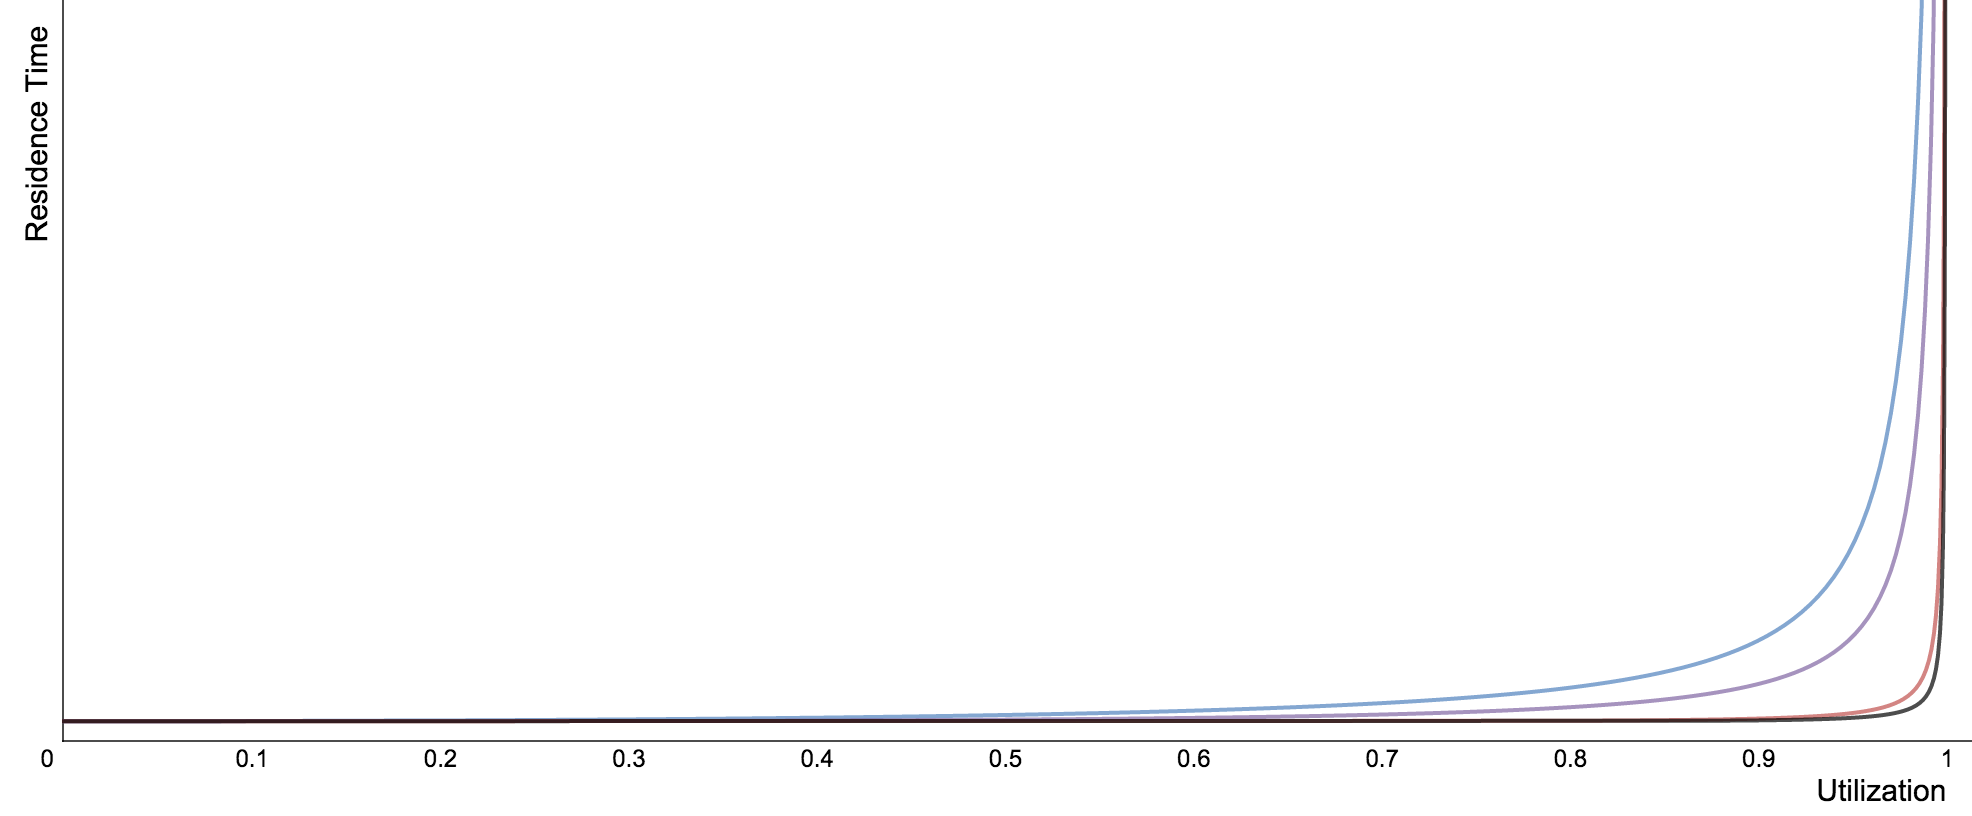
\includegraphics[width=.75\linewidth]{queueing-theory/multi-q}
\end{center}

This chart plots the response time curves of a systems with 1, 2, 4, 32, and 64 servers. The many-server curves remain flat far longer than the others. You can explore this chart on \href{https://www.desmos.com/calculator/iwaj9vujiu}{Desmos} if you like.

The chart also illustrates a rule of thumb you'll probably hear a lot in certain circles: the ``knee'' of the response time curve.\footnote{The location of the ``knee'' is completely arbitrary. The only non-arbitrary definition I've seen is Cary Millsap's, which states that the knee is where the curve is tangent to a line extended from the origin. In general, the knee is actually an \href{http://perfdynamics.blogspot.com/2008/03/watching-your-knees-and-queues.html}{optical illusion}.} It is often said that the knee is at 75\% utilization, and you shouldn't run your servers past that or performance will be bad. The chart illustrates why this folklore is wrong. The knee depends on the configuration. For example, if it's a computer server with 64 processors, you'd be severely underutilizing it if you only ran it at 75\% CPU utilization.

As an aside, one of the biggest wins we see for our customers at VividCortex is giving {\itshape developers} production visibility into database performance. This creates immense efficiency because it breaks down silos of access to information about database performance. That removes a bottleneck in the DevOps ``queueing system'' of engineers and operators communicating with each other, and creates huge return on investment.

\section{Tradeoffs Between Cost and Quality of Service}

Queueing theory explains why there's a difficult, nonlinear tradeoff between
cost and quality of service. If you're in charge of the servers (for example,
purchasing phone lines and hiring staff for a call center), you want to make
sure you don't overprovision, because that's wasteful. On the other hand, you
also don't want to underprovision, because that'll frustrate your customers.

The balance between cost and quality of service is usually considered in one of
three ways:

\begin{enumerate}
\item {\bfseries Quality Driven}. If quality of service is the priority, then
you provision lots of extra capacity in order to get it. You might do this when
realtime response is required for special purposes, for example.
\item {\bfseries Efficiency Driven}. If you care most about efficiency, then you
provision as much capacity as you need, and customers have terrible wait times.
You might do this if you're planning the call center staffing for an airline or
insurance company's customer service line. Just as a random example.
\item {\bfseries Quality and Efficiency Driven}. If you want to balance quality
and efficiency, you aim for this, often abbreviated the QED regime.
\end{enumerate}

It's not difficult to figure out how many servers you need for the quality or
efficiency goals. The QED regime is a bit trickier, though.

It turns out that there's a really neat approximate solution that works very
well in the real world and is useful to help develop your intuition further.
It's typically called the {\itshape square root staffing rule}. In a nutshell,
it says that {\bfseries the spare capacity needed to deliver a given quality of
service grows proportionately to the square root of the traffic.}

As a thought experiment, imagine that you have 10 web servers behind a load
balancer, each of them 80\% utilized. You don't know exactly what performance an
end user experiences, but you're satisfied with it. You expect traffic to triple
for the holiday season. How many servers do you need?

To solve this problem, note that you effectively have 8 servers fully utilized
and 2 servers of spare capacity. Your 8 servers need to triple, and your spare
capacity needs to grow by a factor of \( \sqrt{3} \). So the answer is \( 24 +
2*\sqrt{3} \), or 27.46. You should round this up to the nearest whole server,
or 28 servers.

This rule of thumb is great for developing intuition about how capacity,
utilization, and quality of service grow with traffic. It gets more accurate as
the offered load grows, and works best above a load of 5 or so.

If you want to solve for a specific desired quality of service, that's also
simple. The references at the end of this book contain more information about
this.

\section{Applying Queueing Theory in the Real World}

Many books on queueing theory have extensive examples and problem sets. This is nice, but in my personal experience, I have found queueing theory, especially Erlang queueing models, very difficult to apply to analysis of real systems.

As an example, I've tried to use Erlang formulas when capacity planning for database servers. I got absolutely nowhere because I found it impossible to measure service times. Not only did I not know $S$, but I could not compute utilization, nor could I validate that service times were exponentially distributed,\footnote{The dirty little secret of service times is that they usually seem to be log-normal or gamma distributed, if they even have a clean unimodal distribution at all.} so I wasn't sure the Erlang C model was really the right one to use.

None of this is to say that queueing theory isn't practical. It's enormously practical, but sometimes it's either overkill or there are roadblocks to applying it.

To sum up, queueing theory can be hard to apply for the following reasons:

\begin{itemize}
\item Lack of visibility into what kind of queuing systems lie inside ``black box'' systems
\item Inability to measure and validate inputs and preconditions for a model, particularly service times
\item The difficulty of computing the Erlang formulas
\item Dirty or noisy systems, or poor measurements, that don't seem to conform to models
\end{itemize}

So what is queueing theory good for, then?

In my opinion, queueing theory is best applied {\itshape conceptually} in day-to-day life. That is, it's a great framework for having intelligent opinions and discussions about how systems will behave, because as Neil Gunther says, ``Common sense is the pitfall of performance analysis.'' Queueing theory helps you understand whether things are likely to perform worse than intuition suggests. And when you find such a situation, it might help explain why.

I have applied queueing theory in some real-life use cases. For example, \href{https://www.vividcortex.com/blog/2013/04/17/how-does-adaptive-fault-detection-work-does-it-really-eliminate-thresholds/}{VividCortex's Adaptive Fault Detection algorithm} is based, in part, on queueing theory. But even in that example, queueing theory was more of a conceptual framework for a successful approach to the problem, than an analytical solution to it.

My approach to queueing theory might not match everyone's, but that's why I wrote this book.

\section{Conclusions}
Queueing theory has many practical and important results, as I've
illustrated. In my opinion, however, the most important outcomes of
studying queueing theory are the following:
\begin{itemize}
\item Learning to see queueing systems everywhere. Especially in human systems and the design of teams, processes, and flow of tasks and communications.
\item Building better intuition about which variables influence queueing the most. It's hard to think about nonlinear systems, but if you know they're really sensitive to small changes in particular variables or in specific ranges of values, you'll be better equipped.
\item Understanding the different queueing configurations and their behaviors.
\item Understanding which relationships are linear and straightforward (Little's Law, Utilization Law, etc) and which depend on subtle aspects of system behavior such as arrival processes and their probability distributions.
\end{itemize}
If you reach the end of this book and understand only the following big-picture points, I'll be more than satisfied:
\begin{quote}	% Compile quote
To reduce queueing and waste, work to reduce utilization and variability, increase the number of servers, and avoid specialization.
\end{quote}
This is not everything there is to know about queueing theory, but in my opinion it's everything you need to know.

\section{Further Reading}

This book isn't meant to stand on its own. You should use it as a jumping-off
point for doing further research. Here's a selection of the best reference
material I've found.

\begin{itemize}
\item {\itshape Fundamentals of Queueing Theory} by Gross \& Harris.
\item {\itshape Practical Queueing Analysis} by Mike Tanner.
\item {\itshape Analyzing Computer System Performance With Perl::PDQ} by Neil
Gunther, which despite its name is much more about queueing theory than about
Perl.
\item For more on the QED regime and the square-root staffing rule, see
\href{http://www.columbia.edu/~ww2040/HalfinWW1981.pdf}{Heavy-traffic limits for queues with many exponential servers} by Halfin \& Whitt (1981), or a more recent paper, \href{http://www.columbia.edu/~ww2040/shorter041907.pdf}{What You Should Know About Queueing Models To Set Staffing Requirements in Service Systems}, by Ward Whitt.
\item For more on approximations to the Erlang formulas, see
\href{https://github.com/VividCortex/approx-queueing-theory}{this GitHub
repository}.
\end{itemize}

\newpage

\begin{about}	% Build "About VividCortex"
VividCortex is a SaaS database performance monitoring. The database is the heart of most applications, but it's also the part that's hardest to scale, manage, and optimize even as it's growing 50\% year over year. VividCortex has developed a suite of unique technologies that significantly eases this pain for the entire IT department. Unlike traditional monitoring, we measure
and analyze the system's work and resource consumption. This leads directly to better performance for IT as a whole, at reduced cost and effort.
\end{about}
\makeresources	% Build "Related Resources"
\end{document}
